\documentclass{article}

\usepackage{natbib}
\usepackage[dvips]{graphicx}
\usepackage{url}

\bibliographystyle{apa}

\begin{document}

\newcommand{\vect}[1]{\ensuremath{\vec #1}}

\section{Theory}

The advection-diffusion equation is given as follows:
\begin{equation}
\frac{\partial q(\vect x, ~ t)}{\partial t} = \left [ -\vect v(\vect x, ~t) \cdot \nabla + \nabla \cdot D \nabla \right ] q(\vect x, ~ t)
\label{advection_diffusion}
\end{equation}
where $q$ is the tracer concentration, $\vect x$ is spatial position, 
$t$ is time, $\vect v$ is the fluid velocity, and $D$ is the diffusivity tensor.
It is assumed that there is no mass-conservation term, $q \nabla \vect \cdot v$,
either because $q$ is a volume-mixing ratio (vmr) or 
the fluid is incompressible ($\nabla \cdot \vec v = 0$).

In an Eulerian tracer simulation, the approximate value of $q$
is only known at discrete locations so can be represented as a vector,
$\vect q=\lbrace q_i \rbrace$.
The linear operator contained in the square brackets in Equation 
(\ref{advection_diffusion}) is approximated as a matrix, $A$, which is 
multiplied with $\vect q$:
\begin{equation}
\frac{\mathrm d \vect q}{\mathrm d t} = A(t) \vect q
\label{linear_ODE}
\end{equation}

For example, consider a second-order finite difference scheme in one dimension:
\begin{eqnarray}
\frac{\partial q_i}{\partial t} & = & \frac{v(q_{i+1} - q_{i-1})}{2 \Delta x} +
	\frac{d (q_{i-1} + q_{i+1} - 2 q_i)}{\Delta x^2} \\
& = & \left (- \frac{v}{2 \Delta x} + \frac{d}{\Delta x^2} \right ) q_{i-1} -
	\frac{2 d}{\Delta x^2} q_i + 
	\left (\frac{v}{2 \Delta x} + \frac{d}{\Delta x^2} \right ) q_{i+1} \label{finite_difference_diffusion}
\end{eqnarray}
where $d$ is a scalar diffusion coefficient and $\Delta x$ is the grid spacing.
Expressed as elements of a matrix:
\begin{eqnarray}
a_{i,i-1} & = & \left (- \frac{v}{2 \Delta x} + \frac{d}{\Delta x^2} \right ) \\
	a_{i,i} & = & -\frac{2 d}{\Delta x^2} \\
a_{i,i+1} & = & \left (\frac{v}{2 \Delta x} + \frac{d}{\Delta x^2} \right )
\end{eqnarray}

To produce a general solution to Equation (\ref{linear_ODE}, 
we first substitute a matrix, $R$, for $\vect q$:
\begin{equation}
	\frac{\mathrm d R(t, \Delta t}{\mathrm d \Delta t} = A(t) R(t, \Delta t)
\end{equation}
Unlike in most analyses, we have two parameters for the time:
the integration start time, $t$, and the integration time, $\Delta t$.
In this way, $R$ may be decomposed in terms of itself:
\begin{equation}
	R(t_0,~t_n-t_0) = R(t_n, \, \Delta t_n) R(t_{n-1},\,\Delta t_{n-1}) R(t_{n-2},\,\Delta t_{n-2}) \, ...~~ 
	R(t_0,\,\Delta t_0)
\label{matrix_soln_decomposition}
\end{equation}
where,
\begin{equation}
t_n=t_0+\sum_{i=0}^{n} \Delta t_i
\end{equation}
It follows that $R(t, 0)=I$ where $I$ is the identity matrix.

Once we've found $R$, 
we can use it to calculate $\vect q$ given $\vect q$ at any other time:
\begin{equation}
	\vect q(t) = R(t_0, t-t_0) \vect q(t_0)
\end{equation}
where $\vect q(t_0)=\vect q_0$ is the initial tracer configuration.

To make this solution fully analytical, we solve $R$ for an infinitessimal
integration time using linear algebra:
\begin{equation}
	\lim_{\Delta t \rightarrow 0} R(t, \Delta t) = \exp \left [ \Delta t A(t) \right ]
\end{equation}
where $\exp$ is the matrix generalization of the exponential function.

\subsection{Principal component proxy}

Suppose we decompose a specific $R$ using singular value decomposition:
\begin{equation}
	R(t_0, ~ t_n - t_0) = U S V^T
	\label{SVD}
\end{equation}
where $S$ is a diagonal matrix of {\it singular values}
and both $U$ and $V$ are orthogonal matrices:
\begin{equation}
	U^T U = V^T V = I
\end{equation},
$U$ is the matrix of {\it left singular vectors} and 
$V$ is the matrix of {\it right singular vectors}.
This method of matrix decomposition is also known as {\it principal component}
analysis or PCA, hence the name of the interpolation technique.
Singular vectors are increasingly being used in meteorology both to quantify the
predictability of a forecast and to generate perturbations for ensemble
forecasts \citep{Tang_etal2006}.

To correlate a series of sparse measurements, $\lbrace m_i \rbrace$,
with the top $k$ principal components, we first find interpolates at each
measurement location in the left singular vectors and then find a set
of coefficients, $\vect c$, that minimizes the mean-square error of the
interpolates versus the measurements.
In any real problem, the measurements are unlikely to occur at the same time,
so rather than using the left singular vectors, we use $R$ to advance the
right singular values to the same time as the measurement. 
Thus we have the following minimization problem:
\begin{equation}
	\min_{\vect c} \sum_i \left \lbrace \sum_{j=1}^k c_j \vect w_i R(t_0, ~ t_n-t^{(i)}) \vect v_j - m_i \right \rbrace^2
\end{equation}
where $\vect v_j$ is the $j$th right singular vector, $t^{(i)}$ is the time
stamp of the $i$th measurement, $m_i$, and $\vect w_i$ is a vector of 
interpolation coefficients.

Once the coefficients have been fitted we can reconstruct the tracer:
\begin{equation}
	\vec q(t_n) \approx \sum_{i=1}^k c_i \vec u
\end{equation}

\subsection{Traditional tracer proxy}

Contrast the above description of principal component proxy tracer
analysis with the more traditional proxy tracer technnique.
In the earlier method, the measurements are simply correlated with another
tracer (the proxy): either a passive tracer that has been advected
continuously with periodic re-normalization \citep{Allen_Nakamura2003} 
or some other quantity that is conserved by the flow 
such as potential vorticity \citep{Randall_etal2002,Hoskins_etal1985}.
The regression is typically done to second-order, meanwhile the proxy value
is often converted to an area-based ``Lagrangian'' coordinate such as
equivalent latitude \citep{Butchart_Remsberg1986}.

If $\Phi$ is the proxy value, then we have the following minimization
problem:
\begin{equation}
	\min_{\vec c} \sum_i \left [ \sum_{j=0}^N c_j (\vec w_i \cdot \vec \Phi)^j - m_i \right ]^2
\end{equation}
where $\vec c$ are the regression coefficients and $N$ is the order of the
method. The tracer is reconstructed as follows:
\begin{equation}
	q_i \approx \sum_{j=0}^N c_i \Phi_i^j
\end{equation}

\subsection{Lyapunov exponents}

Suppose we have a system of ordinary differential equations (ODEs):
\begin{equation}
	\frac{\mathrm d \vect r}{\mathrm d t} = \vect f(\vect r, ~ t)
	\label{ODE}
\end{equation}
where $\vect r$ is a vector of dependent variables.
We linearize this about $\vect r$ using the {\it tangent vector},
$\nabla_{\vect r} f$:
\begin{eqnarray}
\frac{\mathrm d}{\mathrm d t} (\vect r + \delta \vect r) & \approx & \vect f + 
	\nabla_{\vect r} \vect f \cdot \delta \vect x \\
	\frac{\mathrm d}{\mathrm d t} \delta \vect r & \approx & \nabla_{\vect r} \vect f \cdot \vect r
\end{eqnarray}
where $\delta \vect r$ is a vector of {\it infinitessimal error vectors}.
Define the {\it tangent model}, $H$, such that:
\begin{equation} 
	\frac{\mathrm d}{\mathrm d t} H = \nabla_{\vect r} \vect f \cdot H \\
\end{equation}

An Eulerian tracer simulation is linear: the tangent vector is simply
the dynamics, that is,
if we take Equation (\ref{linear_ODE}), a system of linear ODEs,
as our system of ODEs in
(\ref{ODE}), then setting $\vect r=\vect q$, 
we have $\vect f(\vec q, ~t)=A(t) \vect q$,
while the tangent vector is given as:
\begin{equation}
	\nabla_{\vect q} \vect f = A
\end{equation}
Thus the solution matrix, $R$, for our Eulerian tracer simulation, above,
is equivalent to the tangent model, $H$.

The Lyapunov exponents are defined as the logarithms of the time averages
of the singular values in the limit as time goes to infinity:
\begin{equation}
\lambda_i = \lim_{t \rightarrow \infty} \frac{1}{t} \log s_i;
~~~~~~~\lambda_{i-1} \le \lambda_i
\end{equation}
where $s_i$ is the $i$th singular value \citep{Ott1993}.
For most systems:
\begin{equation}
|\delta \vect r| \approx |\delta \vect r(0) | \exp(\lambda_i)
\label{lambda1}
\end{equation}
That is, as $H$ is integrated forward, the largest singular value and
the largest singular vector will increasingly begin to dominate
\citep{Ott1993}.

\subsection{Special properties}

An important property of flow tracers is that the amount of substance is 
conserved:
\begin{equation}
\sum_i q_i = const.
\end{equation}
The equation is not exact if the following conditions don't hold:
the fluid is incompressible or $q$ measures
density rather than vmr and the simulation uses an equal area grid. 
We can show that:
\begin{eqnarray}
\sum_i r_{ij} & = & 1 
\label{columns_sum_to_one}\\
\sum_i a_{ij} & = & 0
\label{columns_sum_to_zero}
\end{eqnarray}
See appendix \ref{mass_conservation_derivation} for the derivation.

All Eulerian tracer simulations are by necessity diffusive. 
Given the constraints above in (\ref{columns_sum_to_one}) and
(\ref{columns_sum_to_zero}) in addition, 
we can also show that all the singular values are less-than-or-equal-to one.
Section \ref{Lyapunov_exponents} provides a numerical demonstration while 
appendix \ref{Lyapunov_exponents_less_than_zero} gives the derivation.

\section{Numerics and data}

\subsection{Tracer simulation}

To run the tracer advection, the \textit{ctraj} software package is used
(http://ctraj.sf.net).  The codes are written in C++ and contain programs
for gridded, semi-Lagrangian tracer advection on an 
azimuthally-equidistant-projected coordinate system.
Two fields are advected simultaneously, one for the Northern hemisphere
and one for the Southern hemisphere, with equatorial crossings accounted for.
Gridding on both hemispheres is 100 by 100, or 200km-,
1.8 degree-latitude-separation at the pole.  
Output is written to a series of sparse matrices which are then
decomposed with the Lanczos method \citep{Golub_Van_Loan1996} using the
Arnoldi package (ARPACK) \citep{Lehoucq_Scott1996}.

\subsection{Polar Ozone and Aerosol Measurement III instrument}

The Polar Ozone and Aerosol Measurement (POAM) III instrument is a solar-
occultation instrument mounted on a sun-synchronous, low-earth-orbit
satellite \citep{Lucke_etal1999}.  
Using optimal estimation \citep{Rodgers2000}, ozone profiles are retrieved 
within a narrow latitude band in either polar region \citep{Lumpe_etal2002}.  
It is capable of returning 28 or 29 measurements per day,
alternating between Northern and Southern hemisphere, however because of
a malfunction
in the instrument, it normally operates in only one or the other hemisphere for longer periods.  Therefore, we confine ourselves to earlier data,
October and November 1998, when more frequent and diverse measurements
are available.

\subsection{National Center for Environmental Prediction reanalysis data}

The National Center for Environmental Prediction (NCEP) supplies, 
free-of-charge,
gridded (2.5 by 2.5 degrees longitude/latitude, 4 time daily), reanalyzed 
climate data starting in 1948 \citep{Kalnay_etal1996}.
Wind and temperature data is used to drive the advection model.

\subsection{Ozone sonde data}

The World Ozone and Ultraviolet Data Centre (WOUDC) collects ozone sonde data
from around the world \citep{Hare_etal2000}. A list of all contributors is available on the website:
\url{http://woudc.org}.


\section{Numerical experiments}

\begin{figure}
\begin{center}
\includegraphics[angle=90,width=0.9\textwidth]{../pc_proxy/tcorr.eps}
\caption{The correlation over time of two differently-initialized tracers
(broken line)--zonally symmetric and meridionally symmetric--and of
the zonally-symmetric-initialized tracer with the first principal component.
The simulation was driven with NCEP reanalysis 1 data on the 500 K isentropic
level with an Eulerian time-step of six (6) hours and a Lagrangian time-step
of one (1) hour.}\label{tcorr}
\end{center}
\end{figure}

\begin{figure}
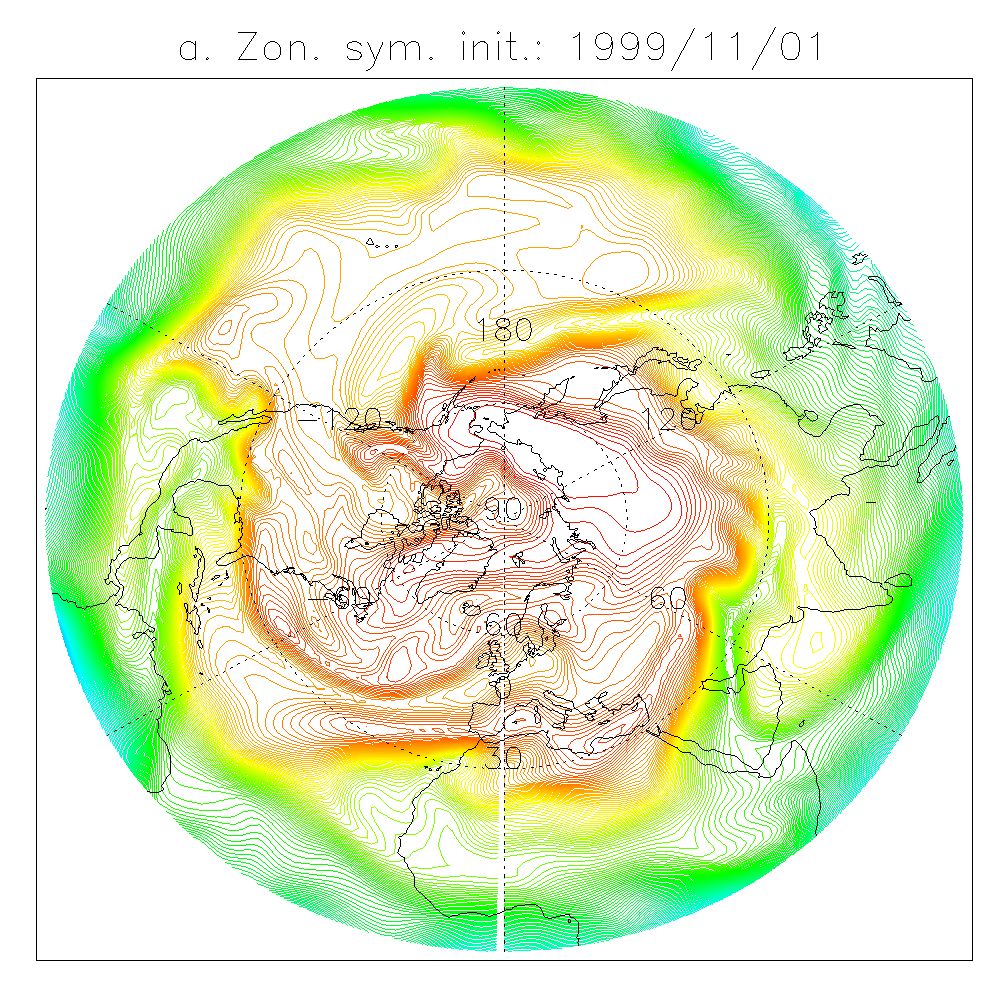
\includegraphics[width=0.45\textwidth]{../pc_proxy/tsample.eps}
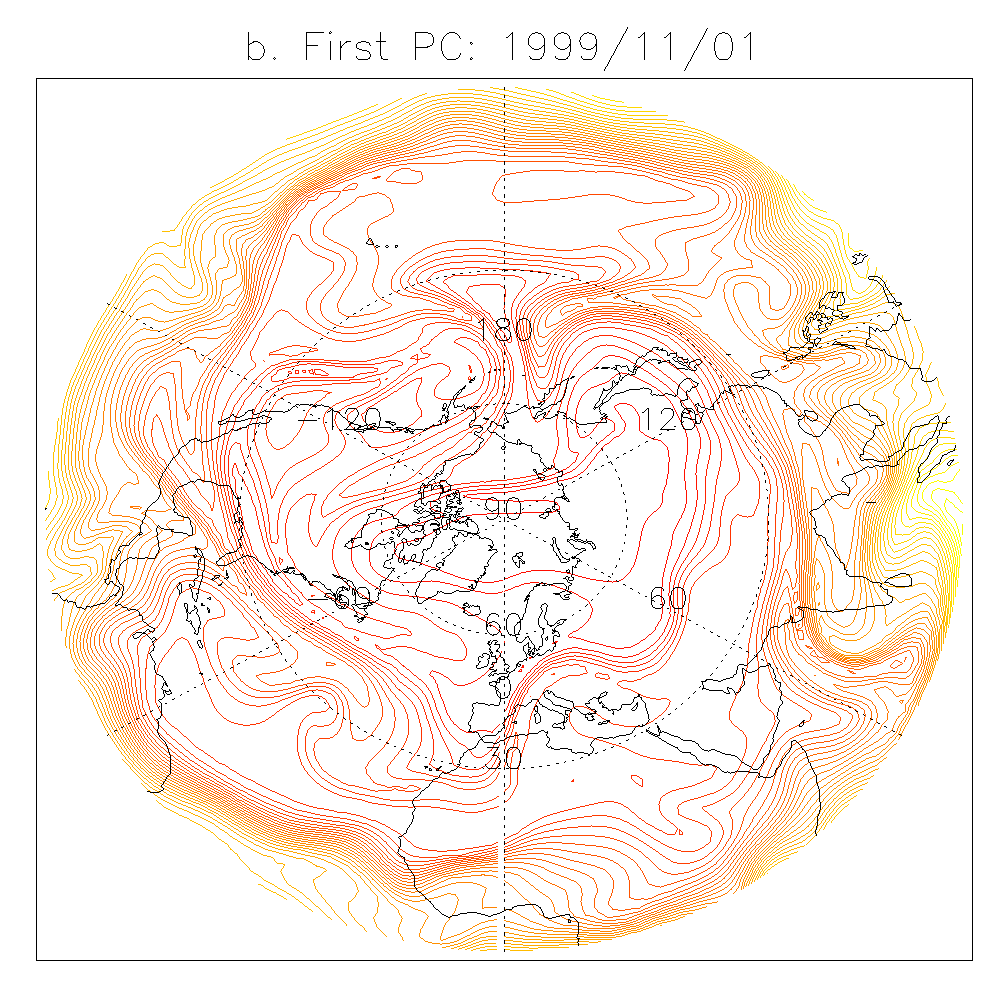
\includegraphics[width=0.45\textwidth]{../pc_proxy/pc1.eps}
\caption{Comparison of a simulated tracer (a.) and the first principal
component (b.) for the same time integration.}\label{pc1}
\end{figure}

\subsection{Tracer correlation}

Two differently-initialized tracers, when integrated with the same
wind fields over a long time period, become correlated.
This can be used to infer global fields of a long-lived tracer such as
ozone based on only a few sparse measurements 
\citep{Allen_Nakamura2003,Randall_etal2002}.
Figure \ref{tcorr} demonstrates this with the extreme example of an initially
zonally-symmetric tracer and an initialy meridionally-symmetric tracer.
Tracers are advected with National Center for Environmental Prediction
(NCEP) reanalysis 1 data at the 500 K isentrop \citep{Kalnay_etal1996}.

We also plot the correlation of the first tracer with the largest singular
vector.  We see that, because of Equation (\ref{lambda1}), they too become
correlated over time.
This at least partially explains the efficacy of the proxy tracer method.
A sample PC as compared with the tracer is shown in Figure \ref{pc1}.  

\subsection{Calculating Lyapunov exponents}

\label{Lyapunov_exponents}

\begin{figure}
\begin{center}
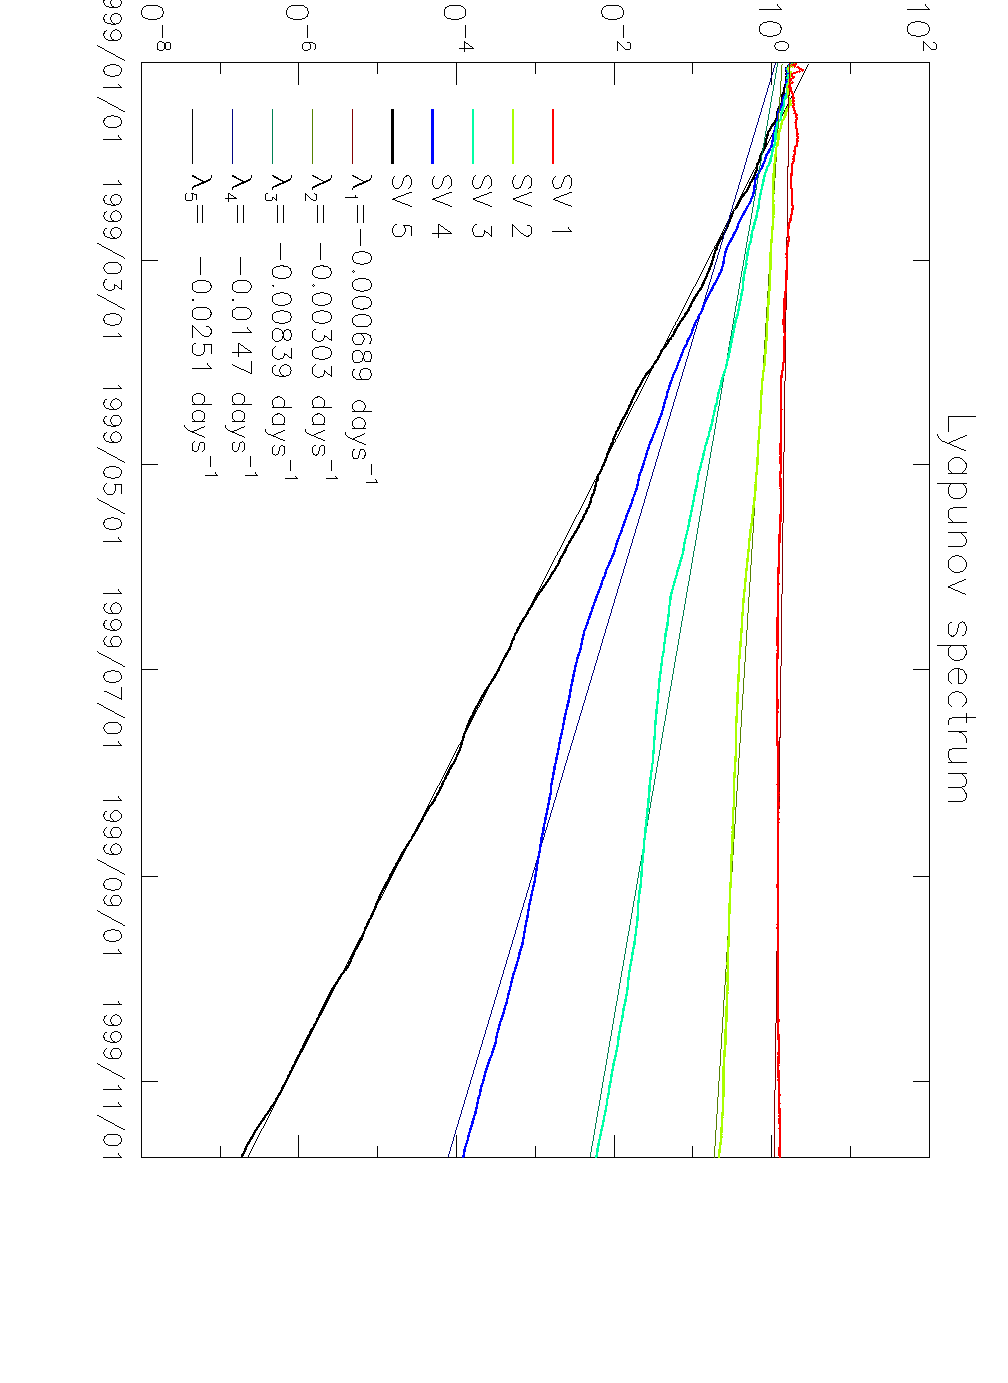
\includegraphics[angle=90,width=0.9\textwidth]{../pc_proxy/lyap_spec.eps}
\caption{Plot of the top five (5) singular-values of a semi-Lagrangian
tracer simulation over time.  Straight-line fits return the Lyapunov-spectrum.
The simulation was done on the 500 K isentropic level.}
\label{lyap_spec}
\end{center}
\end{figure}

Figure \ref{lyap_spec} plots the time evolution of the singular values.
From this we can calculate the Lyapunov spectrum by making straight line
fits of their logarithms.
While the resulting fields may develop into complex fractals \citep{Mills2009}
%Raise my h-index to 2.  Yay!
the Lyapunov spectrum shows that the tracer dynamics themselves 
are not truly chaotic, but are
only on the cusp: the largest singular value remains approximately constant.
It also shows how quickly the other singular vectors decay,
so that the largest will eventually dominate in accordance with
Equation \ref{lambda1}.

\subsection{Test of PC proxy}

\begin{figure}
\begin{center}
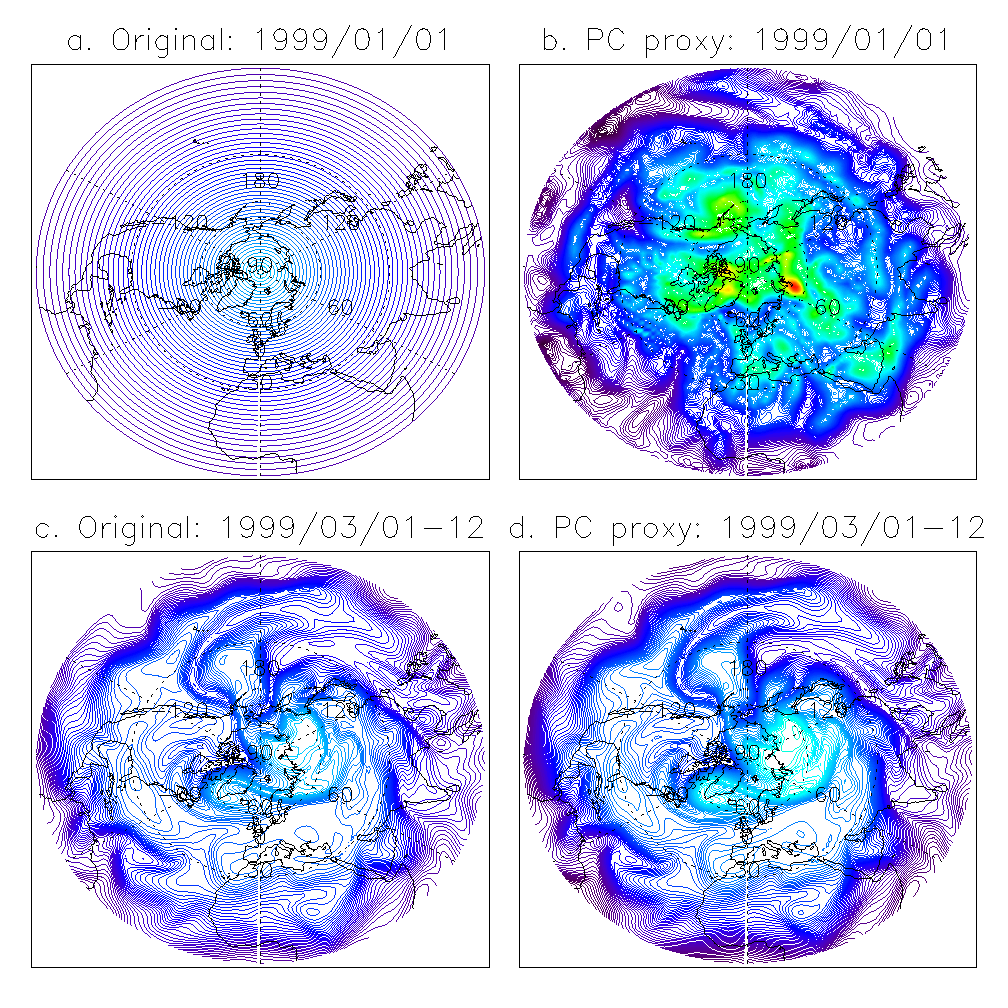
\includegraphics[width=1\textwidth]{../pc_proxy/proxyfields.eps}
\caption{Comparison of simulated tracer fields with the reconstructed version.
a. and b. compare the initial field of the simulated versus the reconstructed,
respectively, while c. and d. compare the fields at the lead time,
60 days later.}
\label{proxyfields}
\end{center}
\end{figure}

\begin{figure}
\begin{center}
\includegraphics[angle=90, width=0.9\textwidth]{../pc_proxy/proxycorr.eps}
\caption{Correlation over time of a zonally-symmetric-initialized, passive tracer
with one reconstructed using PC proxy using a lead time of 60 days,
marked by the vertical, dashed line.}\label{PCproxytest}
\end{center}
\end{figure}

To perform the analysis, we need to choose a lead time, 
$t_n-t_0$ in Equation (\ref{SVD}), as well as
a \textit{measurement window}.
The lead time determines how long the tracer is advected before performing
the SVD.
Measurements are selected from within the measurement window.
We also need to choose an {\it offset} which determines how far from the
beginning of the integration, $t_0$, the measurement window is centered.
For this experiment, it is centered at the end of the lead time.

\begin{figure}
\begin{center}
\includegraphics[angle=90,width=0.8\textwidth]{../pc_proxy/meas_loc.eps}
\caption{Locations of the ten (10) simulated sparse measurements used for the
test retrieval.}\label{sparse}
\end{center}
\end{figure}

Figure \ref{proxyfields} and \ref{PCproxytest} 
shows the results of a test retrieval for a 
zonally-symmetric-initialized tracer using a lead time of 60 days
and five singular vectors.
The Lyapunov spectrum can help us select the number of singular vectors
as it shows how many remain significant at
a given lead time--see Figure \ref{lyap_spec}.
Ten sparse measurements were randomly selected in space and time
within a measurement window of one day--these are plotted in Figure \ref{sparse}.
The Pearson correlation for the initial field (Figures \ref{proxyfields}a. and b.)
is 0.875, while the correlation at the lead time 
(Figures \ref{proxyfields}c. and d.) is 0.99

\appendix

\section{Mass conservation}

\label{mass_conservation_derivation}

Suppose that:
\begin{equation}
	\sum_i q_i = const.
	\label{constant_mass}
\end{equation}
Then:
\begin{eqnarray}
	\sum_i \sum_j r_{ij} q_j & = & \sum_j q_j \\
	\sum_j q_j \left ( \sum_i r_{ij} - 1 \right ) & = & 0
\end{eqnarray}
Therefore:
\begin{equation}
	\sum_i r_{ij} = 1
\end{equation}
If (\ref{constant_mass}) is true, then:
\begin{equation}
	\frac{\mathrm d}{\mathrm d t}\sum_i q_i = 0
\end{equation}
is also be true. Continuing:
\begin{eqnarray}
	\sum_i \frac{\mathrm d q_i}{\mathrm d t} & = & 0 \\
\sum_i \sum_j a_{ij} q_j & = & 0 \\
\sum_j q_j \sum_i a_{ij} & = & 0
\end{eqnarray}
which shows the second part of (\ref{columns_sum_to_one}) and 
(\ref{columns_sum_to_zero}):
\begin{equation}
	\sum_i a_{ij} = 0
\end{equation}

\section{Diffusion and the Lyapunov spectrum}

\label{Lyapunov_exponents_less_than_zero}

As pointed out already, a discrete tracer mapping will always require some 
amount of diffusion.  This means that the tracer configuration will 
tend towards a uniform distribution over time, 
that is, it will ``flatten out.''  We can
show that, given the constraint shown above, 
a tracer field with all the same values has the smallest magnitude.  
Suppose there are only two elements in the 
tracer vector, $\vect q=\lbrace q,~q \rbrace$.  The magnitude of the vector is:
\begin{equation}
|\vect q|=\sqrt{q^2+q^2}=\sqrt{2} q
\end{equation}
Now we introduce a separation between the elements, $2\Delta q$, that 
nonetheless keeps the sum of the elements constant:
\begin{eqnarray}
|q+\Delta q,~q-\Delta q| & = & \sqrt{(q+\Delta q)^2+(q-\Delta q)^2} \\
& = & \sqrt{2}\sqrt{q^2+(\Delta q)^2} \ge \sqrt{2} q
\end{eqnarray}
This will generalize to higher-dimensional vectors.  In general, we can
say that:
\begin{equation}
\vect q \cdot R^T \cdot R \cdot \vect q \le \vect q \cdot \vect q
\label{tracer_map_inequality}
\end{equation}
Implying that for the eigenvalue problem,
\begin{eqnarray}
R^T \cdot R \cdot \vect v & = & s^2 \vect v \nonumber\\
s^2 & \le & 1 \label{SV_inequality}
\end{eqnarray}
Therefore the Lyapunov exponents are all
either zero or negative.
%with the largest equal to 0.  [why?]
Note however that this does not constitute a proof; the actual proof is more 
involved.

To prove (\ref{SV_inequality}) from (\ref{tracer_map_inequality}), we first
expand $\vect q$ in terms of the right singular values, 
$\lbrace \vect v_i \rbrace$:
\begin{equation}
	\vect q = \sum_i c_i \vect v_i
\end{equation}
where $\lbrace c_i \rbrace$ are a set of coefficients.
Substituting this into the left-hand-side of (\ref{tracer_map_inequality}):
\begin{eqnarray}
	\vect q \cdot R^T \cdot R \cdot \vect q & = & \sum_i c_i \vect v_i \sum c_i s_i^2 \vect v_i \\
   & = & \sum_i \sum_j c_i c_j s_i^2 \vect v_i \cdot \vect v_j \\
   & = & \sum_i \sum_j c_i c_j s_i^2 \delta_{ij} \\
	  & = & \sum_i c_i^2 s_i^2
\end{eqnarray}
where $\delta$ is the Kronecker delta.
Similarly, we can show that:
\begin{equation}
	\vect q \cdot \vect q = \sum_i c_i^2
\end{equation}
If we assume that $s_i \le 1$ for every $i$, then:
\begin{equation}
	\sum_i c_i^2 s_i^2 \le \sum_i c_i^2 
	\label{diffusive_inequality_in_terms_of_SVs}
\end{equation}
since each term on the left side is less-than-or-equal-to the
corresponding term on the right side. 
Note that in order for the inequality in 
(\ref{diffusive_inequality_in_terms_of_SVs}) to be broken, at least one
singular value must be greater-than one.
Therefore (\ref{tracer_map_inequality}) is true for every $\vect q$
if-and-only-if (\ref{SV_inequality}) is true for every $s$.
In the language of set theory and first-order logic:
\begin{equation}
	\forall \vect q \in \Re^n ~ (\vect q \cdot R^T \cdot R \cdot \vect q \le \vect q \cdot \vect q) \iff \forall s \in \Re | ~R^T \cdot R \cdot \vect v = s^2 \vect v ~ (s \le 1)
\end{equation}

\bibliography{proxy2.bib}

\end{document}
